\documentclass{bioinfo}
\usepackage{subfigure}
\usepackage{amsmath}
\usepackage[ruled,vlined]{algorithm2e}

\copyrightyear{2012}
\pubyear{2012}

\begin{document}
	\firstpage{1}

	\title[Optimal Interval Intersection Counting]{
	Binary Interval Search (BITS):  \\
	An Optimal Algorithm for Interval Intersection Counting}

	\author[Sample \textit{et~al}]
	{Ryan M. Layer$^1$, 
	Aaron Quinlan$^2$\footnote{to whom correspondence should be addressed},
	Gabriel Robins$^1$, 
	and Kevin Skadron\,$^1$}
	\address{$^{1}$Department of Computer Science, University of Virginia,
	Charlottesville, VA\\
	$^{2}$Department of Public Health Sciences and Center for Public Health
	Genomics, Univeristy of Virginia, Charlottesville, VA}

	\history{Received on XXXXX; revised on XXXXX; accepted on XXXXX}

	\editor{Associate Editor: XXXXXXX}

	\maketitle

	\begin{abstract}
		\section{Motivation:}
		The integration and comparison of diverse genomic datasets is fundamental to
		understanding the biology of the genome and the genetic basis of human disease.
		Researchers must explore many large datasets of genome intervals (e.g., genes,
		polymorphisms, and sequence alignments) in order to place their experiments 
		in a broader context and make new discoveries.  Relationships between experimental
		datasets and genome annotations are typically measured by identifying intervals
		that intersect: that is, they overlap and thus share a common genome interval. 
		Given the continued advances in DNA sequencing technologies, efficient methods 
		for measuring relationships between many, often large, sets of genomic features
		is crucial for future discoveries.

		\section{Results:}
		Here we introduce the Binary Interval Search (BITS) algorithm, a novel and scalable 
		approach to the interval set intersection problem. Our analyses illustrate that BITS 
		is as efficient as existing approaches on a single CPU and outperforms existing methods
		for many common applications. Moreover, we demonstrate that the BITS algorithm is 
		well-suited to parallel computing architectures such as Graphics Processing Units (GPUs), 
		yielding substantial speedups (over ??x) over single CPU implementations. We demonstrate
		the utility of this scalable algorithm for Monte-Carlo measurements of statistical associations 
		between experimental datasets and genomic features. We note that our approach is 
		especially suited to the emerging ``hybrid'' computing cluster nodes equipped with GPU 
		cards to boost computing throughput.

		\section{Availability:} \href{http://bedtools.googlecode.com}{http://bedtools.googlecode.com}

		\section{Contact:} arq5x@virginia.edu
	\end{abstract}

	\section{Introduction}

	Searches for intersecting intervals in multiple sets of genomic features are
	crucial to nearly all genomic analyses. For example, intersection is used to
	compare ChIP enrichment between experiments and cell types, identify potential
	regulatory targets, and compare genetic variation among many individuals.
	Interval intersection is the central operation in a broader class of
	``genome arithmetic'' techniques, and, as such, intersection underlies the
	functionality found in genome browsers~\citep{kent2002,robinson2011} and popular
	analysis software such as SAMTOOLS~\citep{li2009}, BEDTOOLS~\citep{quinlan2010}, 
	GATK~\citep{mckenna2010}, and GALAXY~\citep{giardine2005}.

	Given the importance of interval set intersection to genomic discovery, many
	sequential algorithms have been developed based on trees,
	NCLists~\citep{alekseyenko2007}, or linear sweeps of pre-sorted
	intervals~\citep{richardson2006}. For example, the UCSC genome browser
	introduced a clever scheme based on R-trees that places intervals from one
	dataset into hierarchical ``bins''~\citep{kent2002}.  Intervals from a second
	dataset are then compared to matching bins in order to narrow the search for
	intersections to a focused portion of the genome.  While this popular approach
	is used by the Kent tools software, BEDTools~\citep{quinlan2010}, SAMTOOLS, and
	TABIX, the underlying tree structure demands substantial memory for large
	datasets and is often difficult to parallelize. As an alternative,
	memory-efficient approach, recent versions of BEDTools and other software
	conduct a linear ``sweep'' through pre-sorted datasets while maintaining a
	priority heap to track intersections as they are encountered. While the
	complexity of such sequential sweep algorithms can be shown to be theoretically
	optimal, they are nonetheless difficult to scale to parallel architectures.

	As the throughput of massively parallel DNA sequencing continues to increase,
	the limitations of these traditional approaches to interval intersection become
	increasingly acute. Traditional techniques for measuring gene expression (e.g.,
	microarrays) and chromatin states (e.g., ChIP-chip) are being supplanted by
	sequencing-based techniques (RNA-seq and ChIP-seq, respectively), and
	whole-exome and whole-genome experiments are now routine. Consequently, typical
	genomics labs now conduct analyses including datasets with millions, if not billions 
	of intervals. Experiments of this size require substantial computation time per 
	pair-wise comparison, and a typical analysis requires comparisons to many large
	sets of genomic features. As extant sequential solutions scale poorly 
	and are already reaching their theoretical performance limits, it is clear that 
	parallel approaches must be developed to allow discovery to keep pace with the
	scale and complexity of modern datasets.

	The current generation of Graphics Processing Units (GPUs), such as NVIDA's
	CUDA, can improve performance for the subset of problems that map well to the
	massively parallel single instruction, multiple data (SIMD) architecture.  These
	architectures deploy hundreds of basic parallel processing units, and can
	support thousands of concurrently executing threads.  In order to fully utilize
	the hardware, a problem must be decomposed into many small subtasks.   Problems
	that do not fit this model are less likely to dramatically benefit from GPU
	hardware.

	Neither the linear sweep algorithm nor the existing search algorithms are good
	candidates for the GPU architecture.  Parallel sweep algorithms have been
	proposed~\citep{goodrich1993, kriegel1991, mckenney2009} for segment
	intersection (a generalization of interval intersection), but they depend on a
	partitioned input space scheme that can exploit only limited parallelism.
	Search algorithms, where one set is a list of interval queries and the other set
	is an interval database, can leverage a higher degree of parallelism by
	performing searches concurrently.  However, the database generation can be even
	slower than the searching itself, and may be difficult to parallelize. 
	\textbf{TODO: this feels a bit weak}

	In this manuscript we introduce the Binary Interval Search (BITS) algorithm 
	as a new and scalable solution to the fundamental problem of interval set 
	intersection.  Our algorithm is optimal in the sequential case, avoids slow 
	linear sweeps, does not require \emph{ad hoc} data structures, and maps well 
	to parallel architectures.  The BITS algorithm is based on the novel 
	observation that the size of the intersection between two sets can be directly 
	computed without the need to enumerate each intersection. For each interval 
	in the query list, two binary searches are performed to determine the number 
	of intervals in the database that intersect the query interval.  Each pair of searches 
	is independent, and thus all the searches can be performed in parallel.  This type of 
	algorithm is perfectly suited to GPU-type architectures that are optimized 
	for large numbers of threads.

	Our analysis shows that the parallel BITS algorithm, when applied to a GPU
	architecture, can provide substantial (over 75X) speedups over other widely-used
	sequential interval intersection approaches. These results are particularly
	promising for applications that require large numbers of intersection
	operations, such as database searches and Monte Carlo simulations.


	\subsection{The Interval Set Intersection problem}
	Before we describe our parallel set intersection algorithm, we review some basic
	definitions.  A genomic interval is a single continuous stretch of a genome with
	a start and end location (e.g., a gene), and a genomic interval set is a
	collection of genomic intervals (e.g., all known genes).  More generally, an
	interval is the set of all numbers between a start value and an end value, that
	can be represented as the pair $(a.start, a.end)$.  Two intervals $a$ and $b$
	{\em intersect} when $(a.start \leq b.end)$ and $(a.end \geq b.start)$.  The
	intersection of two interval sets $A=\{a_1, a_2, \dots, a_N\}$ and
	$B=\{b_1, b_2, \dots, b_M\}$ is the set of interval pairs:

	\begin{equation*}
		\begin{split}
			\mathcal{I}(A,B)= &\{ <a,b> | a \in A, b \in B, \\
			& a.start \leq b.end \wedge a.end \geq b.start\}
		\end{split}
	\end{equation*}

	Intervals within a set can intersect, but {\em self-intersections} are not
	included in $\mathcal{I}(A,B)$.  The interval set intersection problem is a
	special case of the segment intersection problem where all points are located on
	the same line, and each segment belongs to one of two sets.

	There are four natural sub-problems for interval set intersection, listed here
	in order of increasing generality and complexity.
	\begin{enumerate}
		\item The {\em decision problem} $\mathcal{I_D}(A,B)$:  given interval sets $A$
		an $B$, does there exist and interval in $A$ that intersects and interval in
		$B$?
		\item The {\em counting problem} $\mathcal{I_C}(A,B)$: how many pair-wise
		intersections exist between the intervals $A$ and $B$?
		\item The {\em per-interval counting problem} $\mathcal{I_P}(A,B)$: how many
		intervals in $B$ intersect each interval in $A$?
		\item The {\em enumeration problem} $\mathcal{I}(A,B)$: what is the total set of
		pair-wise intersection between $A$ an $B$?
	\end{enumerate}

	\subsection{Related Work}

	Most interval set intersection algorithms use either a linear sweep to scan the
	intervals in both sets, or search for intersections using a pre-computed data
	structure.

	\subsubsection{Linear Sweep Algorithms}

	\textbf{TODO: cite Richardson, BEDTOOLs, BEDOPS}
	
	In general, the linear sweep algorithm combines intervals from $A$ and $B$ into
	a single set $S$, and the elements in $S$ are then processed in order.  An {\em
	active structure} tracks intervals as they enter and exit the ``context'', and
	two intervals intersect if and only if they are in context at the same time.

	To correctly track the intervals that are in context, all segment starts, ends,
	and intersections behind the sweep must be known.  McKenny and McGuire~\citep{mckenney2009} 
	proposed that segments be broken at the partition boundaries, which effectively 
	resets the sweep invariant between partitions.   The broken segments are re-joined 
	in the final result.  Although partitioning allows for some amount of parallel
	execution, the level of parallelism that is possible in linear sweep algorithms 
	is limited to the number of partitions that can be created, which is a function 
	of how the segments are distributed, not the size of the segment set.

	\subsubsection{Searching algorithms}
	
	\textbf{TODO: cite Richardson, BEDTOOLs, BEDOPS}
	
	An alternative to the linear sweep involves searching for intersections.  Given
	two interval sets $A$ and $B$, $B$ is treated as a database of intervals, and
	$A$ is utilized as set of query intervals.  For each interval $a_i \in A$, the
	search returns the set of intervals in $B$ that intersect $a_i$.

	The correctness of the searching algorithm is complicated by a subtle detail.
	If the intervals in $B$ are sorted by their starting positions, then a binary
	search of $B$ for the query interval end position $a_i.end$ will return the
	interval $b_j \in B$, where $b_j$ is the last interval in $B$ that starts before
	interval $a_i$ ends.  This would seem to imply that if $b_j$ does not intersect
	$a_i$, then no intervals in $B$ intersect $a_i$, and if $b_j$ does intersect
	$a_i$, then other intersecting intervals in $B$ could be found by scanning the
	intervals starting before $b_j$ in decreasing order, stopping at the first
	interval that does not intersect $a_i$.  However, as shown in Figure~\ref{fig:contained} 
	this technique is complicated by the possibility of intervals wholly {\em contained} 
	inside other intervals.

	\begin{figure}[h]
		\centering
		\subfigure[The search for $y$ in the database returns interval $h$, which does
		not intersect $y$.  All preceding intervals must be scanned to ensure
		correctness.]{
		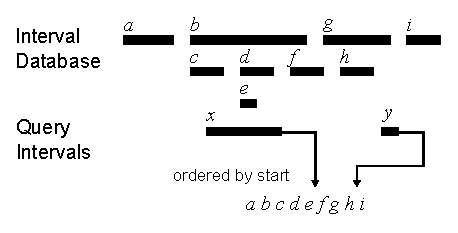
\includegraphics[width=3in]{figures/bits1.eps}
		\label{fig:contained}
		}
		\subfigure[Two lists, one sorted by start and the other by end, can be used to
		find the size of the intersecting set without enumerating the intersecting
		intervals.]{
		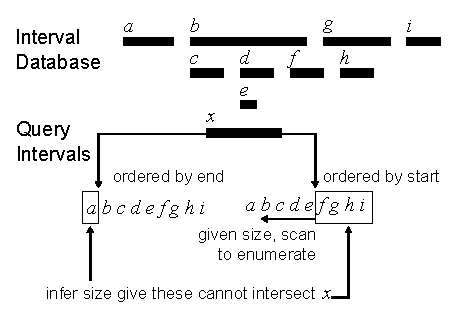
\includegraphics[width=3in]{figures/bits2.eps}
		\label{fig:bits}
		}
		\caption{Contained intervals complicate intersection searches.
		A single list \subref{fig:contained} does not allow for
		efficient searching because all prior intervals must be scanned for
		correctness. Two lists \subref{fig:bits} can be used to
		find the intersecting set size.}
		\label{bitssearching}
	\end{figure}

	An interval $b_j\in B$ is ``contained'' if there exists an interval
	$b_k \in B$ where $b_k.start \leq b_j.start$ and $b_j.end \leq
	b_k.end$.  Considering such intervals, if the interval found in the
	previous binary search $b_j$ does not intersect the query interval
	$a_i$, we cannot conclude that no interval in $B$ intersects $a_i$,
	because there may exist an interval $b_{j-x} \in B$ where $b_{j-x}.end
	> a_i.start$.  Furthermore, if $b_j$ does intersect $a_i$, then the
	subsequent scan for other intersecting intervals cannot stop at the
	first interval that does not intersect $a_i$; it is possible that some
	earlier containing interval intersects $a_i$. Therefore, the scan is
	forced to continue until it reaches the beginning of the list.

	Search algorithms can expose a higher degree of parallelism by
	allowing each thread to handle one interval query, making it possible
	for the parallelism to be proportional to input size, rather than to
	the distribution of intervals within the input space.  This level of
	parallelism may not be possible using existing sequential search
	algorithms, due to their reliance on methods and secondary structures
	that do not map well onto massively parallel architectures.

% METHODS

	\section{Methods}
	\subsection{Binary Interval Search (BITS) Algorithm}
	We now introduce our new Binary Interval Search (BITS) algorithm for solving
	the interval set intersection problem.  The key observation underlying the BITS 
	algorithm is that the size of the intersection between two sets can be 
	determined without \emph{enumerating} each intersection.  For each interval 
	in the query set, two binary searches are performed to determine the \emph{number} 
	of intervals in the database that intersect the query interval.  Each pair of
	searches is independent of any others, and thus all searches can be
	performed in parallel.  

	Our algorithm uses a different, but equivalent, definition of interval
	intersection.  Previously, the intersecting set was defined as the set
	of intervals in the interval database $B$ that end after the query
	interval $a_i$ begins, and which begin before $a_i$ ends.  However,
	contained intervals make it difficult to find this set directly.  The
	search for the intersecting intervals can start at the interval in $B$
	closest to $a_i$, but must continue to the beginning of $B$ because
	there is no condition indicating that all intersecting intervals have
	been found.  By restating the intersection definition, we are able to
	determine the size of the intersecting set, which provides a
	terminating condition for the search, so that it may stop once the
	last interval in the intersecting set has been found.

	We define the set of intervals $\mathcal{I}(B,a_i) \in B$ that
	intersect query interval $a_i\in A$ to be the intervals in $B$ that
	are not in either the set of intervals that end before $a_i$ begins,
	or in the set of intervals that start after $a_i$ ends.  That is:
	\begin{equation*}
		\begin{split}
			\mathcal{L}(B,a_i) = &\{b\in B| b.end < a_i.start\} \\
			\mathcal{G}(B,a_i) = &\{b\in B| b.start > a_i.end\} \\
			\mathcal{I}(B,a_i) = &B / (\mathcal{L}(B,a_i) \cup \mathcal{G}(B,a_i))
		\end{split}
	\end{equation*}

	Finding the intervals in $\mathcal{I}(a_i,B)$ for each $a_i\in A$ by
	taking the difference of $B$ and the union of $\mathcal{L}(B,a_i)$ and
	$\mathcal{G}(B,a_i)$ is not efficient.  However, we can quickly find
	the size of $\mathcal{L}(B,a_i)$ and the size $\mathcal{G}(B,a_i)$,
	then infer the size of $\mathcal{I}(B,a_i)$.  With the size of
	$\mathcal{I}(B,a_i)$, we can directly answer the decision problem, the
	counting problem, and the per-interval counting problems.  Moreover,
	the size can also serve as the previously missing terminating
	condition in the enumeration problem.

	\begin{algorithm}[h]
		\DontPrintSemicolon
		\footnotesize
		\KwIn{Sorted interval starts and ends $B_S$ and $B_E$, query interval $a$}
		\KwOut{Number of intervals $c$ intersecting $a$}
		\BlankLine
		\textbf{Function} \textsc{ICount}$(B_S,B_E,a)$
		\Begin {
		$first \gets \textsc{BSearch}(B_S, a.end)$\;
		$last \gets \textsc{BSearch}(B_E, a.start)$\;
		$c \gets first - last$\;
		\Return $c$\;
		}
		\caption{Single interval intersection counter}
	\end{algorithm}

	\begin{algorithm}[h]
		\DontPrintSemicolon
		\footnotesize
		\KwIn{Database intervals array $B$ and query interval array $A$}
		\KwOut{Number of intersections $c$ betweeen $A$ and $B$}
		\BlankLine
		\textbf{Function} \textsc{Counter}$(A,B)$
		\Begin {
		$B_S \gets [b_1.start, \dots, b_M.start]$ where $|B| = M$\;
		$B_E \gets [b_1.end, \dots, b_M.start]$ where $|B| = M$\;
		\textsc{Sort}($B_S$)\;
		\textsc{Sort}($B_E$)\;
		$c \gets 0$\;
		\For{$i \gets 1$ \KwTo $|A|$} {
		$c \gets c + \textsc{ICount}(B_S,B_E,A[i])$
		}
		\Return $c$\;
		}
		\caption{Interval intersection counter}
	\end{algorithm}

	\begin{algorithm}[h]
		\DontPrintSemicolon
		\footnotesize
		\KwIn{Database intervals array $B$ and query intervals array $A$}
		\KwOut{Array of intersections counts $C$ where $|C|=|A|$}
		\BlankLine
		\textbf{Function} \textsc{PerIntervalCounter}$(A,B)$
		\Begin {
		$B_S \gets [b_1.start, \dots, b_M.start]$ where $|B| = M$\;
		$B_E \gets [b_1.end, \dots, b_M.start]$ where $|B| = M$\;
		\textsc{Sort}($B_S$)\;
		\textsc{Sort}($B_E$)\;
		$C \gets [0, \dots, 0]$\;
		\For{$i \gets 1$ \KwTo $|A|$} {
		$C[i] \gets \textsc{ICount}(B_S,B_E,A[i])$
		}
		\Return $C$\;
		}
		\caption{Per interval intersection counter}
	\end{algorithm}

	\begin{algorithm}[h]
		\DontPrintSemicolon
		\footnotesize
		\KwIn{Database intervals array $B$ and query intervals array $A$}
		\KwOut{Array of pair-wise intersections $E$ }
		\BlankLine
		\textbf{Function} \textsc{Enumerator}$(A,B)$
		\Begin {
		$B_S \gets [b_1.start, \dots, b_M.start]$ where $|B| = M$\;
		$B_E \gets [b_1.end, \dots, b_M.start]$ where $|B| = M$\;
		\textsc{Sort}($B_S$)\;
		\textsc{Sort}($B_E$)\;
		$C \gets \textsc{PerIntervalCounter}(A,B)$\;
		$R \gets \textsc{PrefixSum}(C)$\;
		$E \gets [<0,0>, \dots, <0,0>]$\;
		$start \gets 0$\;
		\For{$i \gets 1$ \KwTo $|A|$} {
		$end \gets R[i]$\;
		$from \gets \textsc{BSearch}(B_S, A[i].end)$\;
		\While{$end - start > 0$}{
		\If{ $A[i]$ intersects $B[from]$}{
		$E[start] = <A[i], B[from]>$\;
		$start \gets start + 1$\;
		}		
		$from \gets from - 1$\;
		}
		}
		\Return $E$\;
		}
		\caption{Intersection enumerator}
	\end{algorithm}


	The core function in our algorithm 
	$\textsc{ICount}(B_S,B_E,a_i) = |\mathcal{I}(B,a_i)|$ determines the number of
	intervals in the database $B$ that intersect query interval $a_i$.  As shown in
	Figure~\ref{fig:bits}, $B$ is split into two integer lists 
	$B_S = [b_1.start, b_2.start, \dots, b_M.start]$ and 
	$B_E = [b_1.end, b_2.end, \dots, b_M.end]$, then $B_S$ and $B_E$ are sorted
	numerically.  Next, two binary searches are performed,
	$first=\textsc{ BSearch}(B_S, a_i.end)$ and 
	$last=\textsc{ BSearch}(B_E,
	a_i.start)$.  Since $B_S$ is a sorted list of each interval start coordinate in
	$B$, the elements greater than or equal to $first$ in $B_S$ correspond to the
	set of intervals in $B$ that start after $a_i$ ends.  Similarly, the elements
	less than or equal to $last$ in $B_E$ correspond to the set of intervals in $B$
	that end before $a_i$ starts.  From these two values, we can infer the size of
	the set $\mathcal{I}(B,a_i)$:
	\begin{equation*}
		\begin{split}
			|B|-first=&|\mathcal{G}(B,a_i)| \\
			last=&|\mathcal{L}(B,a_i)| \\ 
			|B|-(last+(|B|-first))=&|\mathcal{I}(B,a_i)|
		\end{split}
	\end{equation*}

	This problem cannot be solved with a single sorted list because
	contained intervals prevent the total ordering of $B$.  If $B$ is
	sorted by interval start coordinates, then the interval end
	coordinates may be unordered and $last$ can not be found
	efficiently.  Similarly, if $B$ is sorted by interval end,
	$first$ can not be found efficiently.  With the subroutine
	$\textsc{ICount}(B_S,B_E,a_i)$ thus defined, the four interval set intersection
	problem variants can now be solved:

	\begin{enumerate}

		\item
		{\em Decision problem:} Let $c$ be an accumulator variable that is
		initialized to zero; then for each $a_i \in A$, accumulate $c = c +
		\textsc{ICount}(B_S,B_E,a_i)$.  If $c\ne0$ then return {\em yes}, otherwise
		return {\em no}.

		\item
		{\em Counting problem:}  Let $c$ be an accumulator variable that is
		initialized to zero; then for each $a_i \in A$, accumulate $c = c +
		\textsc{ICount}(B_S,B_E,a_i)$.  The total accumulated count $c$ is returned.

		\item
		{\em Per-interval counting problem:} Let $C$ be an accumulator
		array where element $C[i]$ corresponds to the number of
		intersection for each element in $a_i\in A$.  Fore each $a_i \in A$,
		set $C[i]=\textsc{ICount}(B_S,B_E,a_i)$.  The total list of counts $C$ is then
		returned.

		\item
		{\em Enumeration problem:}
		First find the per-interval counting array $C=\textsc{PerIntervalCounter}(A,B)$
		then the let $R$ be the prefix sum of $C$. The array $R$ is used to track the
		number of intervals that must be found in each of the subsequent scans.  Let
		$start = 0$ track the number of enumerated intersections.
		For $i=1\dots|A|$, let $end = R[i]$ where $end - start$ is the nubmer intervals
		in $B$ that intersect $a_i$.  Let $from=\textsc{BSearch}(B_S, a_i.end)$ be
		the initial position of the scan.  While $end - start > 0$ some number of
		intervals in $B$ must be scanned for an intersection with $a_i$.  If $a_i$
		intersections $b_from$ then let $E[start] = <a_i, b_from>$ and 
		$start=start+1$.  Then let $from = from +1$.  Finallty the total set of
		intrsecting intervals $E$ is returned.
	\end{enumerate}

	\subsection{Time Complexity Analysis}

	To compute $\textsc{ICount}(B_S,B_E,a_i)$ for each $a_i$ in $A$, the interval
	set $B$ is first split into two sorted integer lists $B_S$ and $B_E$,
	which requires $O(|B| \log |B|)$ time.  Next, each instance of
	$\textsc{ICount}(B_S,B_E,a_i)$ searches both $B_S$ and $B_E$, which consumes
	$O(|A| \log |B|)$ time.  For the counting problems, combining the
	results of all $\textsc{ICount}(B_S,B_E,a_i)$ instances into a final result can
	be accomplished in $O(N)$ time.  The total complexity of the counting
	problems is therefore $O((|A| + |B|) \log |B|)$.

	The enumeration problem requires additional steps to scan the
	intervals in $B_S$.  In the best case scenario, each scan requires
	$\textsc{ICount}(B_S,B_E,a_i)$ extra steps, to a total of $O(|B| \log |B|
	+ C)$ time, where is $C$ is the number of intersections.
	However,
	contained intervals can cause the scan to process more than $C$
	elements.  If there exists some $a_i$ that intersects $b_{j}$ and
	$b_{j-2}$, but not $b_{j-1}$ (i.e., $b_{j-2}$ contains $b_{j-1}$),
	then the enumeration scan will consider one extra element, namely
	$b_{j-1}$.  In the pathological case, $b_0$ contains intervals $\{b_1,
	\dots, b_N\} \in B$, $a_i$ intersects $b_0$, and $a_i$ starts after
	interval $b_N$ ends.  This scenario would cause the enumeration scan
	to consider all the elements in $B$.  If all $a_i$ in $A$ are
	pathological, then each scan would required $|B|$ extra steps, to a
	total of $O(|B| \log |B| + |A||B|)$ time.

	\subsection{Parallelization}

	Performing a single operation independently on many different inputs
	is a classic parallelization scenario.  When based on the subroutine
	$\textsc{ICount}(B_S,B_E,a_i)$, which is independent of all 
	$\textsc{ICount}(B_S,B_E,a_j)$
	for $a_j \in A$ where $i \neq j$, interval set intersection can be a
	{\em pleasingly parallelizable} problem that easily maps to a number
	of parallel architectures.

	\subsubsection{OpenMP}

	A popular option for parallelizing applications is the OpenMP standard.
	Converting a sequential program into a parallel program can be as simple as
	adding a single compiler directive.  We report performance benchmarks using
	OpenMP as a comparison reference when considering alternative parallel
	architectures.

	\subsubsection{CUDA}

	NVIDIA's Compute Unified Device Architecture (CUDA) is a single
	instruction multiple data (SIMD) architecture that provides
	programmers a general interface to a large number of parallel graphics
	processing units (GPUs).

	The BITS algorithm is especially well suited for the NVIDIA CUDA
	architecture for a number of reasons.  First, CUDA is optimized to handle large
	numbers of threads.  By assigning each thread one instance of
	$\textsc{ICount}(B_S,B_E,a_i)$ for all $a_i \in A$, the number of threads will
	be proportional to the file size.  CUDA threads also execute in lock-step and
	any divergence between threads will cause reduced thread utilization.  While
	there is some divergence in the depth of each binary search performed by
	$\textsc{ICount}(B_S,B_E,a_i)$, it has an upper bound of $O(log |B|)$.  Outside of
	this divergence $\textsc{ICount}(B_S,B_E,a_i)$ is a classic SIMD operation.  And
	finally, the only data structure required for this algorithm is a sorted list.
	Sorting on GPU has been an active area of research for many years, and current
	GPU sorting algorithms can sort billions of integers within
	seconds~\citep{merrill2011}.

	\section{Results}

	We compared the performance of the counting, per interval counting, and
	enumeration algorithms (the three most widely used interval intersection
	sub-problems) in BITS to two other popular interval intersection software
	packages, BEDTools~\citep{quinlan2010} and Kent tools~\citep{kent2002}.  While
	BITS maps well to multiple parallel architectures (multi-core CPU using OpenMP,
	and NVIDIA GPU using CUDA), a fair comparison cannot be made between parallel
	BITS and Kent tools or BEDTools because parallel version of these packages are
	not available.  Therefore, we demonstrate the value of our algorithm by
	comparing sequential versions.  We then show the added benefit provided by 
	BITS using parallel architectures.

	The performance of a particular solution may depend on the distribution of
	intervals within the sets.  For example, a solution that places intervals in
	bins may perform poorly when intervals are unevenly distributed across the bins.
	Therefore, each algorithm was evaluated considering three different
	representative interval intersection scenarios, the components of each scenario
	are given in Figure~\ref{distro}:

	\begin{figure}[h]
		\begin{center}
			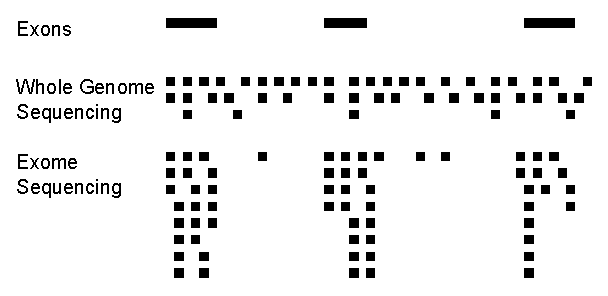
\includegraphics[width=3in]{figures/data_distribution.eps}\end{center}
			\caption{Representative interval intersection scenarios.}
			\label{distro}
		\end{figure}

		\begin{enumerate}
			\item
			{\em Uniform interval distribution}: the intersection between human
			exons and human genome-wide sequencing data.  Despite representing roughly 1
			percent the human genome, exons are evenly distributed throughout the genome.
			Genome-wide sequencing experiments typically produce short sequence intervals
			that are approximately uniformly distributed across the genome. Thus, each exon
			will intersect roughly the same number of sequencing intervals, and a large
			number of sequencing intervals will not intersect an exon.

			\item
			{\em Biased interval distribution}:  the intersection between human
			exons and human exome sequencing data.  By design, exome sequencing experiments
			intentionally focus DNA sequences to the coding exons.  Thus, the vast majority
			of sequence intervals will ``pile up'' in only a few regions (i.e., the exons)
			across the genome. In contrast to the previous scenario, nearly every exon
			interval will have a large number of sequence interval intersections, and nearly
			all sequencing intervals will intersect an exon.

			\item
			{\em Many short intervals}: the intersection between human exome
			sequencing data and human genome-wide sequencing data.  Since both sequencing
			data sets have a large number of short intervals and they are from different
			distributions, there will be a small number of intersections.
		\end{enumerate}

		Both the genome-wide and exome intervals are from the 1000 Genomes Project
		NA12878 individual.  To test scalability, we varied the number of intervals in
		both the exome and genome-wide sets by randomly sampling between $10^4$ and
		$10^7$ intervals.  The human exon data set includes the exons from all RefSeq
		genes, obtained from the UCSC Genome Browser. 

		All run-times were measured on a 2.66 GHz quad-core Intel Xeon X555 CPU with 8
		MB of cache running Ubuntu Linux version 4.4.3 (kernel version 2.6.32-34).
		Run-times for CUDA were measured on an NVIDIA Tesla C2050 GPU with 448 1.15 GHz
		cores, 3 GB of global memory, CUDA driver version 4246739, and CUDA runtime
		version 4.0.  The source code was compiled using gcc version 4.4.3, and NVIDIA
		CUDA compilation tools release 4.0, V0.2.1221.  In each case, run-times measure 
		the performance of the intersection algorithm and thus do not include disk
		reading, writing, or the time required to initialize the GPU.

		The results of our tests are given in Figure~\ref{count},
		Figure~\ref{perintervalcount}, and Figure~\ref{enumerate}.
		
		\textbf{TODO: this sections is incorrect.  Refocus on general equivalence
		and superiority for very large datasets and for biased data.}
		
		In nearly every case, the sequential version of BITS outperformed both Kent
		tools and BEDTools.  The most striking improvement was in the interval counting
		operation, where ---in the largest operation (10M many short intervals, a total
		of 2e$^7$ intervals)--- sequential BITS achieved a speedup of 7.7x over Kent
		tools and 27.4x over BEDTools.  In this same case the speedup over Kent tools
		and BEDTools by OpenMP BITS was 13.1x and 46.6x, and the speedup by CUDA BITS
		was 143.7x and 508.8x, respectively.

		While BITS did have some improvement in enumeration operation, the speedup was
		an order of magnitude lower than in the counting operations, and Kent tools
		performed better than sequential bits in one scenario.  This result is expected
		given that BITS is optimized for counting intersections, which is generally more
		a useful operation in large-scale comparisons.

		\begin{figure}[h]
			\centering
			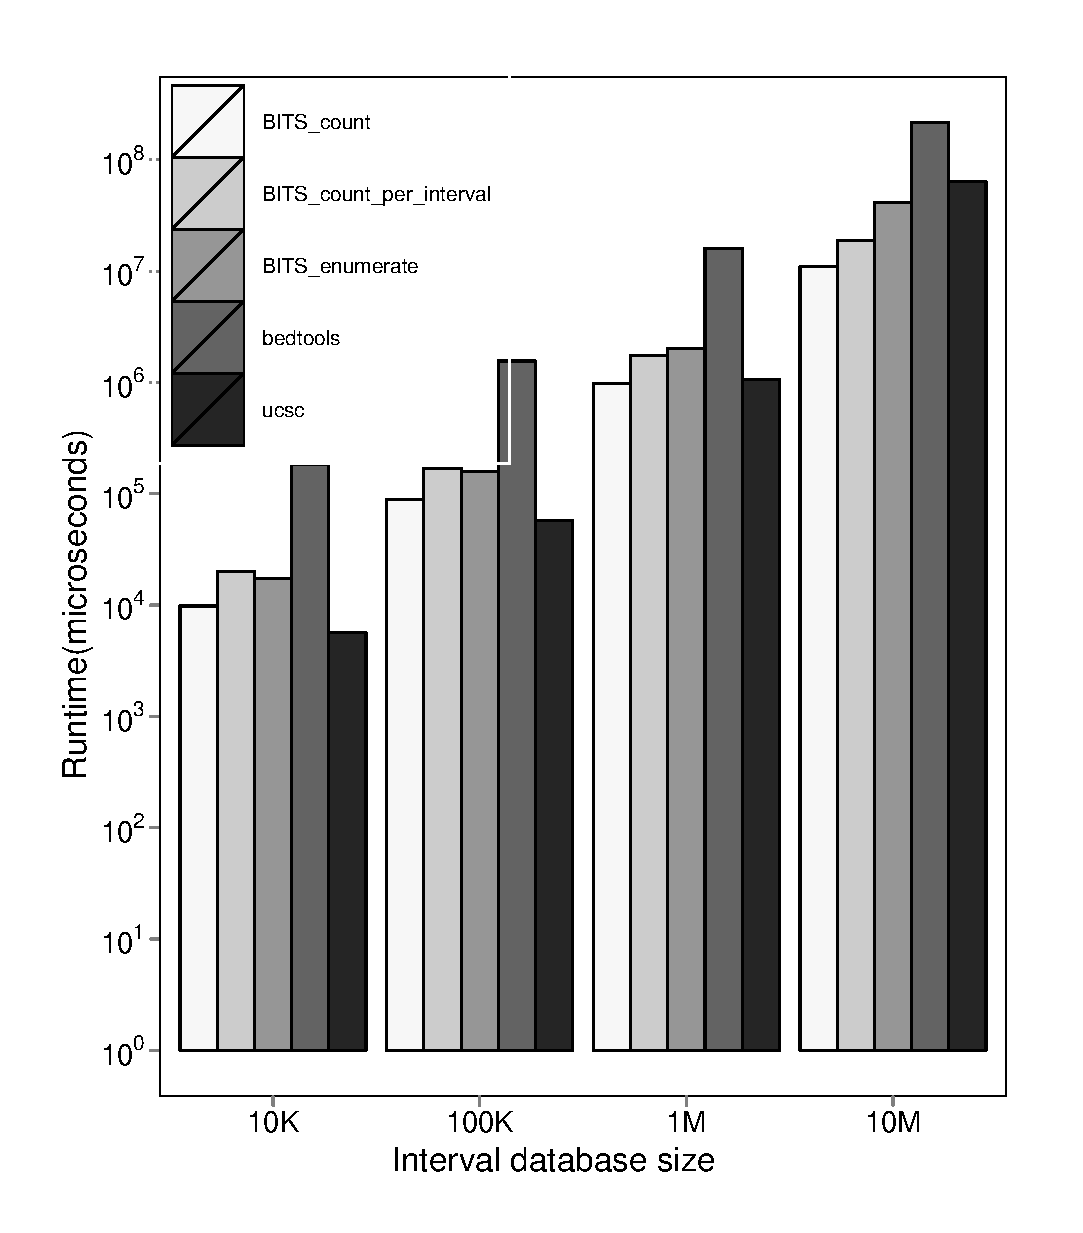
\includegraphics[width=3in]{figures/genome-v-exome.eps}
			\caption[]{Run times for each algorithm using exome and whole-genome datasets (FIX: caption and need error bars).}
		\end{figure}
		
		\begin{figure}[h]
			\centering
			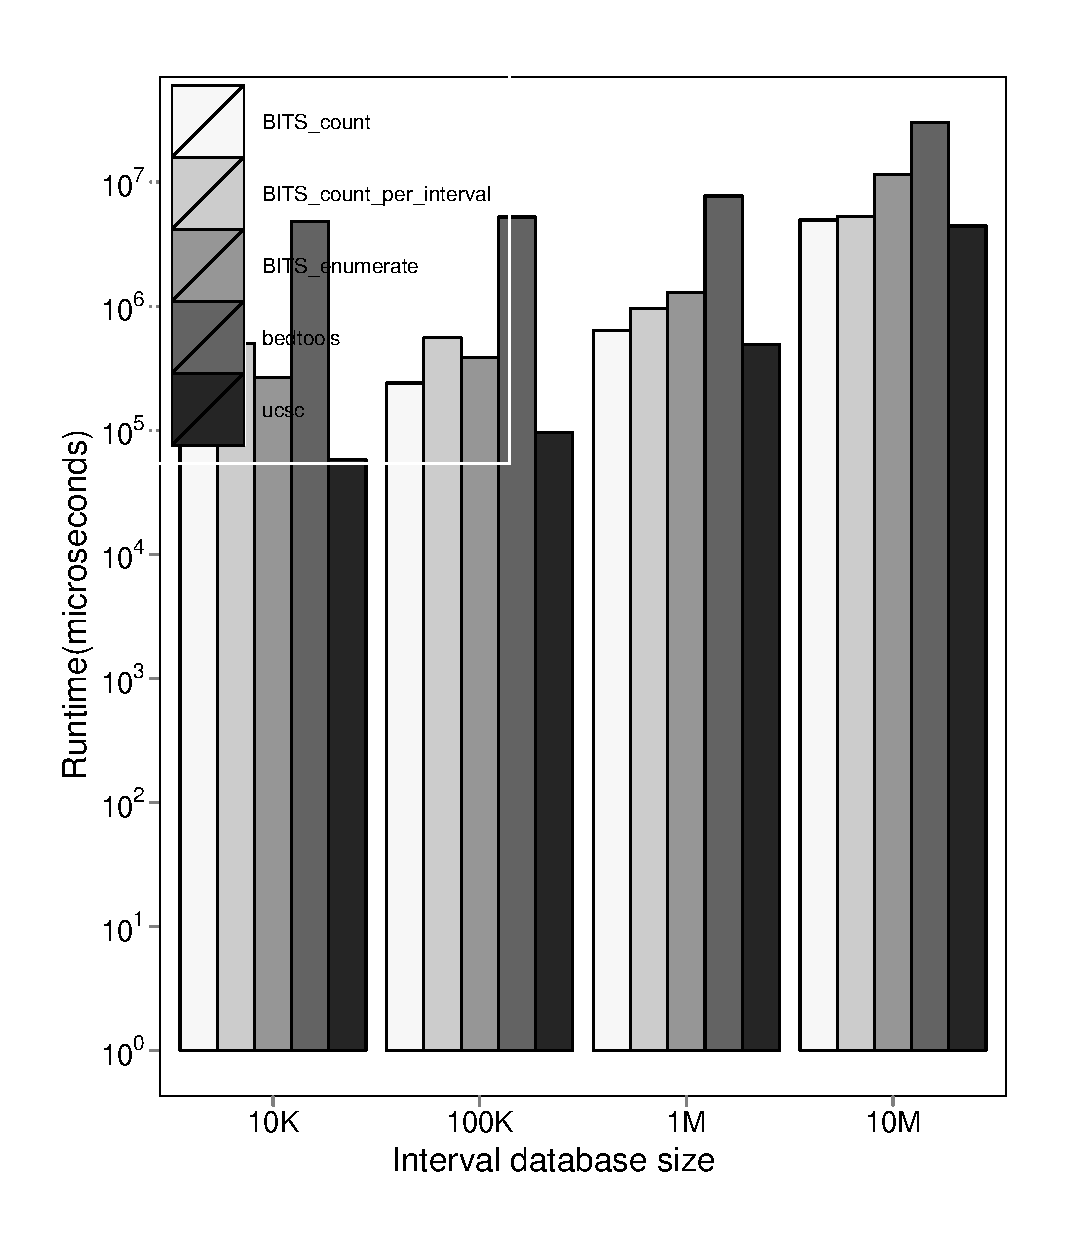
\includegraphics[width=3in]{figures/exons-v-genome.eps}
			\caption[]{Run times for each algorithm using exons and whole-genome datasets (FIX: caption and need error bars).}
		\end{figure}
		
		\begin{figure}[h]
			\centering
			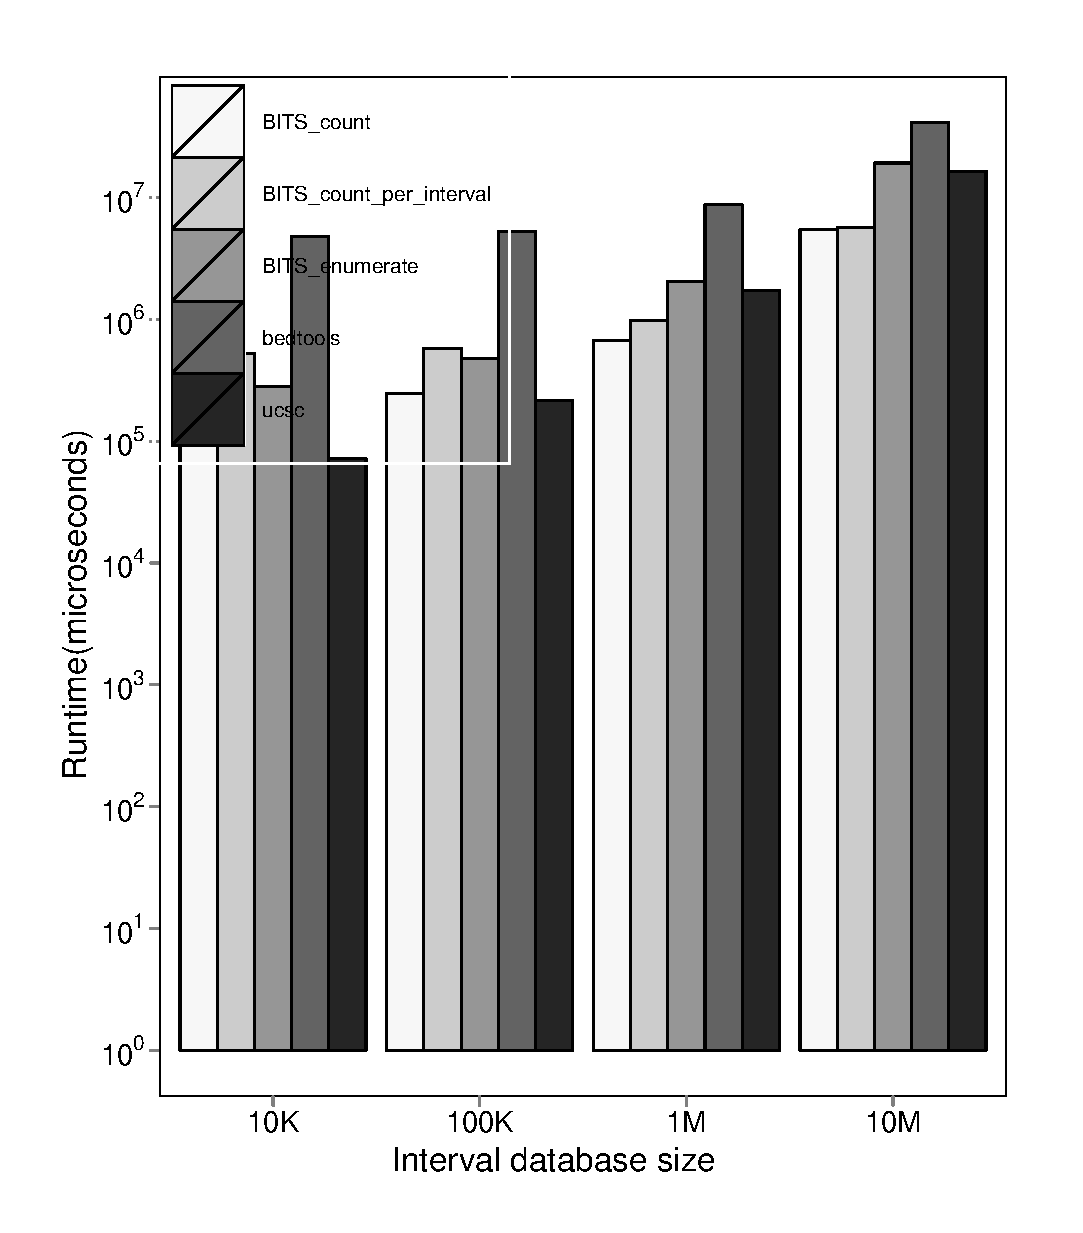
\includegraphics[width=3in]{figures/exons-v-exome.eps}
			\caption[]{Run times for each algorithm using exons and whole-exome datasets (FIX: caption and need error bars).}
		\end{figure}

		The performance profiles of counting (Figure~\ref{count}) and per interval
		counting (Figure~\ref{perintervalcount}) were similar for all algorithms.
		In these two scenarios, excluding the smallest data sets, all versions of BITS
		performed faster than both Kent tools and BEDTools.  For the 10K database, Kent
		tools performed faster than the sequential and OpenMP version of BITS by up to a
		factor of three.  The following table gives the average speedups of the three
		versions of BITS over Kent tools and BEDTools for the 10 million interval
		database.

		%\begin{table}[h]
		%\caption{Average speedup for intersection counting and per interval counting for
		%the 10M database}
		%\centering
		\begin{center}
			\begin{tabular}{lll}
				\\
				& Kent tools & BEDTools \\
				\hline
				Sequential	& 4.5x	& 17.7x \\
				OpenMP		& 11.1x	& 43.1x \\
				CUDA		& 75.8x	& 285.4x \\
				\\
			\end{tabular}
		\end{center}
		%\label{table:avgcp}
		%\end{table}

		For enumeration, the performance improvements of the  sequential and OpenMP
		versions of BITS were an order of magnitude lower against BEDTools, and
		non-existent against Kent tools.  In fact, Kent tools performed better than
		sequential BITS by a factor of nearly three for the smallest database
		(Figure~\ref{fig:eexonfull}), and the run times of the two where nearly
		equivalent for the largest database.  The CUDA version of BITS did provide a
		modest improvement over both Kent tools and BEDTools, but at a level lower than
		in counting and per interval counting.
		The following table  gives the average speedups of the three versions of BITS
		over Kent tools and BEDTools for the 10 million interval database.

		%\begin{table}[h]
		%\caption{Average speedup for intersection enumeration for the 10M database.}
		%\centering
		\begin{center}
			\begin{tabular}{lll}
				\\
				& Kent tools & BEDTools \\
				\hline
				Sequential	& 1.5x & 7.3x \\
				OpenMP		& 1.3x & 6.4x \\
				CUDA		& 3.8x & 24.9x \\
				\\
			\end{tabular}
		\end{center}
		%\label{table:avge}
		%\end{table}

		The fact that BITS performed better in counting than in enumeration is to be
		expected given BITS is based on the observation that counting can be
		performed without enumerating each intersection, and that enumeration in BITS
		first counts the number of intersections then makes a second pass to enumerate.
		While this is a limitation of the BITS algorithm, counting and per interval
		counting are the primary functions used to analyze large data sets.  For
		example, the utility of the full list of 9,148,823 intersection between human
		exon and the exome sequencing of the NA12878 individual (the biased distribution
		scenario) is limited, while the number of intersections per exon can provide
		insight into deletions, duplications, and other properties of NA12878's
		genome.

		\section{Conclusion}
		We have developed a highly scalable approach to interval intersection
		that exploits the speed and simplicity of the binary search. Our 
		binary interval search (BITS) algorithm is founded upon the novel 
		observation that the count of overlapping intervals between two sets 
		can be obtained without the computational burden of enumerating each individual
		intersection. We illustrate that the two binary searches conducted
		against the database for each query interval are independent, and thus, the
		BITS algorithm is well suited for GPU architectures that are optimized for
		large numbers of concurrent threads. Our results with the CUDA architecture
		demonstrate speed increases of up to 143x and 508x relative to existing 
		approaches to genome interval intersection. Using a single CPU, we still observe
		improvements of 17.7x and 49.5x, illustrating the our new approach will benefit
		existing tools that are incapable of exploiting GPU architectures.  This
		substantial performance increase is especially relevant to modern genomic
		analyses given the staggering scale and complexity of current and future
		datasets.  Indeed, given that the BITS algorithm excels at \emph{counting}
		overlaps, it is perfectly suited to address many fundamental yet computationally
		intensive genomic analyses including RNA-seq transcript quantification, ChIP-seq
		peak detection, and searches for copy-number and structural variation.

		We also note that the performance gains that BITS offers increase as the number
		of interval comparisons increases. Therefore, we anticipate that our approach
		will enable previously intractable large-scale comparisons of experimental
		datasets with comprehensive genome annotation databases that contain thousands
		of distinct genome annotation sets. Moreover, this approach is directly amenable
		to Monte Carlo measurements of associations between interval sets, as such
		simulations require thousands of iterations in order to demonstrate
		significance. Given the performance and simplicity of the algorithm, we
		anticipate that it will benefit a wide range of existing tools ranging from
		visualization tools to widely-used genomic analysis software.

		\bibliographystyle{natbib}
		%\bibliographystyle{achemnat}
		%\bibliographystyle{plainnat}
		%\bibliographystyle{abbrv}
		%\bibliographystyle{bioinformatics}
		%
		%\bibliographystyle{plain}
		%
		\bibliography{bioinformatics}
	\end{document}
